\section{Proposed Method}
\label{sec:method}

\begin{figure*}[th]
    \centering
    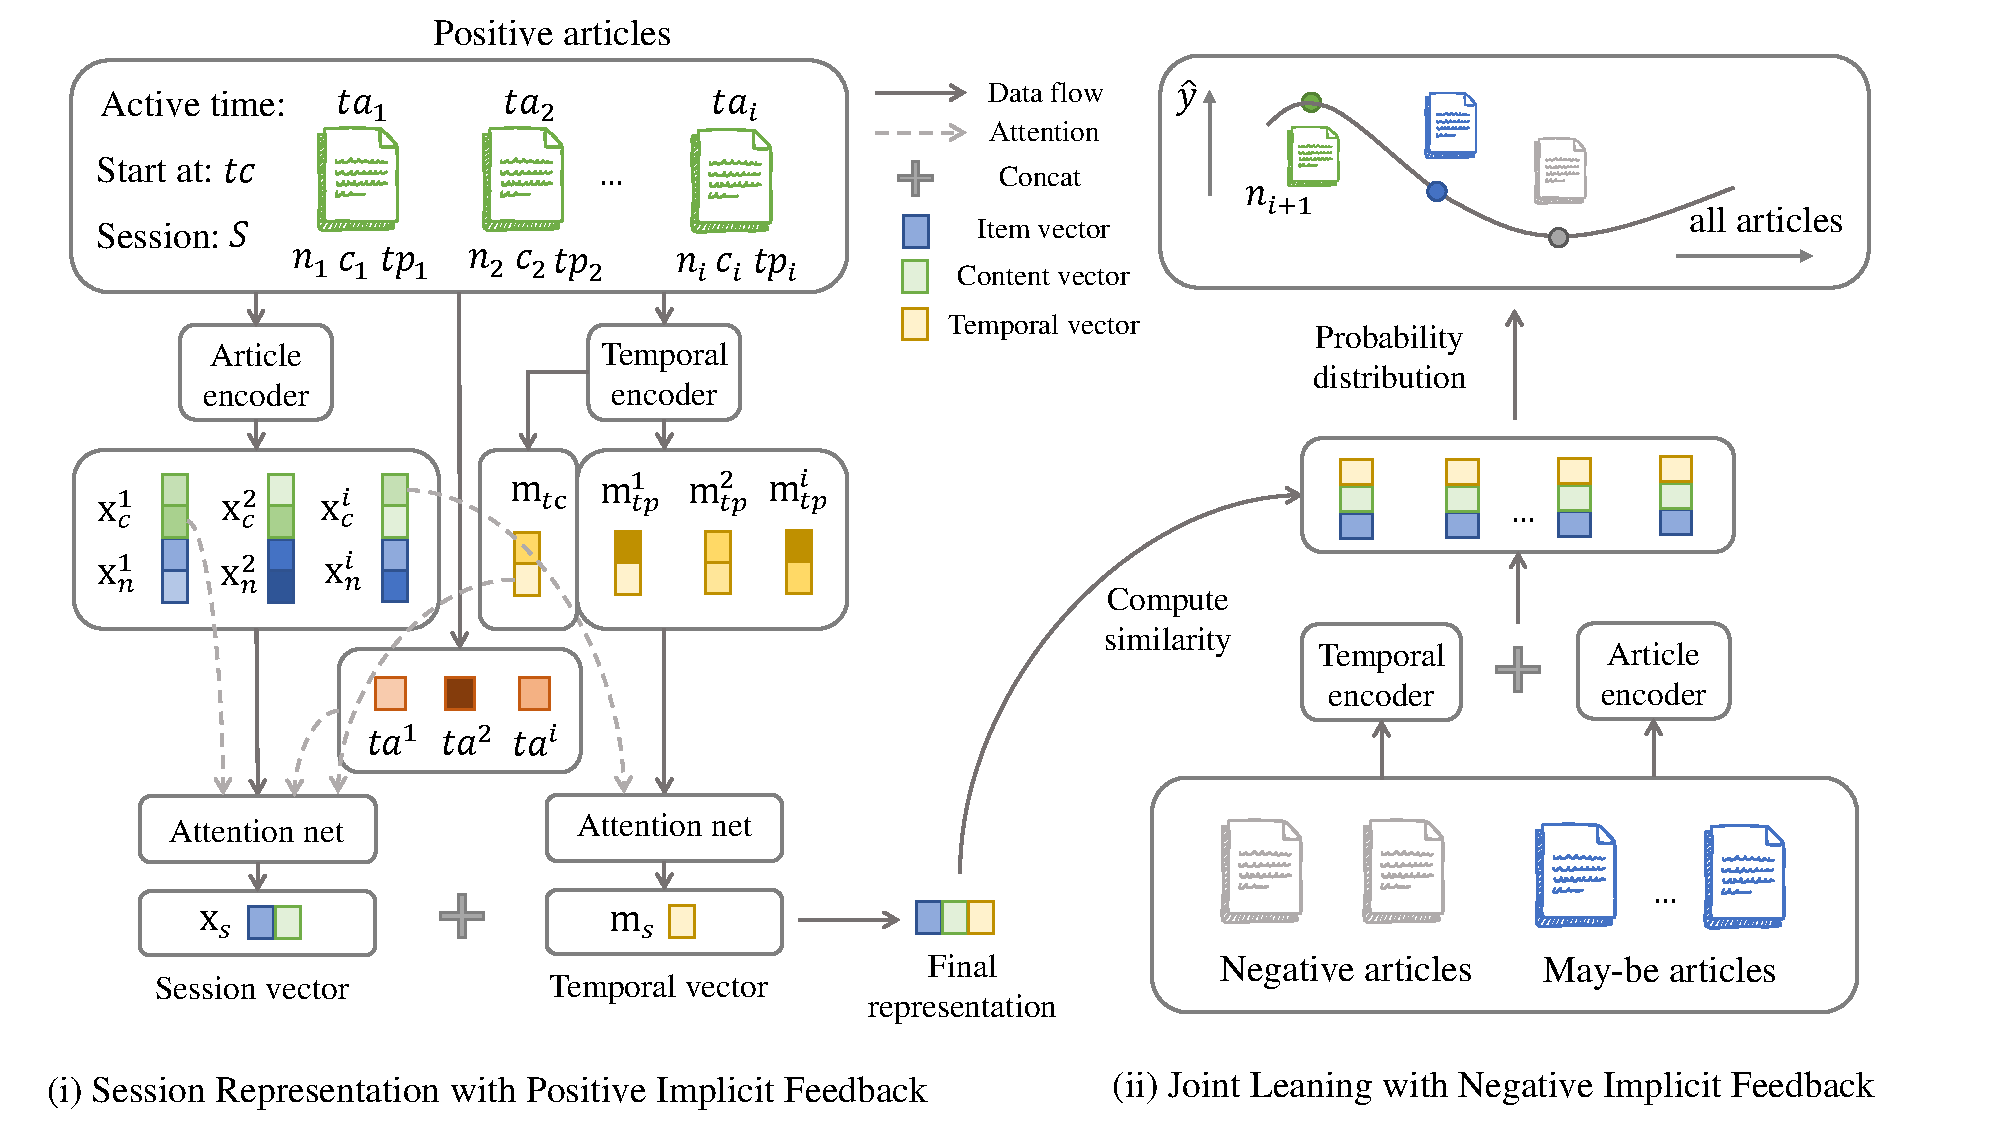
\includegraphics[width=0.85\textwidth]{fig/architecture.pdf}
    \caption{The overview of the two-stage framework.}
    \label{fig:architecture}
    \Description[Architecture]{This is an architecture of ITCAR}
\end{figure*}

In this section, we propose a new session-based news recommendation
framework that leverages implicit-feedback which mainly contains two parts: 
(i) model positive implicit user feedback with the help of news content and 
temporal information; 
and (ii) jointly learn the model using negative implicit feedback.
The high-level overview of ITCAR is illustrated in \figref{fig:architecture}. 
Next we zoom into each of its components of user implicit feedback modeling.

First, we denote each article as a trainable high-dimensional vector 
$\mathbf{x_n}$ to learn articles' sequential relation during training. 
In order to capture the topic-related interests of users and to 
alleviate the article cold-start problem, we introduce a content vector $\mathbf{x_c}$ 
for each article based on article's text (in some datasets, this is the news title). 
These two vectors are concatenated together to represent a clicked article 
in the session. For different clicked articles in a session, 
the user may spend different amounts of time to read them, reflecting their preference
or interest in them. We can model this implicit feedback using the
article's content $\mathbf{x_c}$ and active time $ta$ (time spent on an article) 
to construct a session representation vector $\mathbf{x_s}$. 

Second, we can make better use of the temporal information. 
$tc$ refers to the start time of a session, which may reflect the daily routine behind users. We can assume that users who are reading at the same day of a week or hour of a day have a higher possibility to share the same reading behavior, 
thus we add $tc$ in the calculatation of the session-level personalized attention when 
constructing $\mathbf{x_s}$. 
On the other hand, the publish time $tp$ of each article can also be 
formed into a sequence, which reflects the reading habbits of the user. 
We represent the periodic date information as the hidden vector 
$\mathbf{m_t}$ when training.

Once we successfully model positive implicit feedback using the content and temporal information, in stage two, we jointly train the model with negative implicit feedback. We obtain score distribution through computing similarity between the final session representation vector with hybrid information and the article vectors for all articles in the candidate set. Articles in the impression list not viewed by the user are regarded 
as negative samples, thus we emphasize the negative information of these articles 
through adding penalty loss for high scores on them and jointly train with  the two losses.

\subsection{Session Representation with positive Implicit Feedback}
\label{sec:positive feedback}

\subsubsection{Article encoder}

An article may be consumed by multiple users, and articles may be associated
with each other because they are consumed by the same user in a single session.
We thus build an item embedding vector $\mathbf{x_n}$ to store the hidden information 
of different articles. We first create an item embedding matrix 
$\mathbf{E_n}\in \mathbb{R}^{(N+1)\times d_n}$, 
where $d_n$ is the latent dimensionality, and $N$ is the number of items in the 
training set, and the remaining $1$ dimension is used as the indicator for the item in the test set while not in the training set. Then we retrieve article $n_i$'s embedding vector through $\mathbf{E_n}$ as $\mathbf{x_n}_i$.

Some session-based recommendation systems target only fixed number of items, 
but news articles are published constantly and the number is infinite. 
To deal with the article cold-start problem, it is necessary to consider the 
textual content of articles when recommending~\cite{sottocornola2018session}. 
For article textual content embedding, a common practice today is to use 
pre-trained word embeddings, such as Word2Vec trained from a large text corpus 
of a target language. We average the $d_c$ dimension vector of words in news title, 
to represent the topic-oriented content of articles. Once we get the 
content vector $\mathbf{x_c}_i$ of article $n_i$, 
we concatenate $\mathbf{x_c}_i$ and $\mathbf{x_n}_i$ to encode 
the article as $\mathbf{x_{nc}}_i \in \mathbb{R}^{(d_n+d_c)}$. 

\subsubsection{Session representation}
\label{sec:session}

After the success of Recurrent Neural Network in sequence prediction 
tasks~\cite{hidasi2015session}, 
several recent works show the potential of attention mechanism in 
modeling sequential information in 
recommendation~\cite{kang_self-attentive_2018,liu2018stamp,xu2019time}. 
To model the varying user preference to the articles in the same session,  
we propose an attention network, and use weighted user interests considering the whole session.

We denote $\alpha_i$ as the attention weight of $i$-th articles $n_i$ in session $S_u$. It is calculated by click-level information: 
article vector $\mathbf{x_{nc}}_i$ and content vector $\mathbf{x_{c}}_i$ of $n_i$. 
The attention is computed as follows:
\begin{equation}
    \alpha_i = W_0 \times \sigma (W_1 \times \mathbf{x_{nc}}_i + W_2 \times \mathbf{x_c}_i + b_1),
\end{equation}
\begin{equation}
    \alpha_i = \frac{exp(\alpha_i)}{\sum_{j=1}^{|S_u|}exp(\alpha_j)},
\end{equation}
where $W_0\in \mathbb{R}^{1 \times d_n}, W_1 \in \mathbb{R}^{(d_n+d_c)\times d_n}, W_2 \in \mathbb{R}^{d_c\times d_n}$ are weighting parameters, $b_1\in \mathbb{R}^{d_n}$ is a bias, and $\sigma(\cdot)$ is active function $exp(\cdot)$ is exponential function.

Then we use a feed forward network to compute the final representation $\mathbf{x_s}$ of session $S_u$, which is the summation of article vectors weighted by their attention weights:
\begin{equation}
    \label{eq:final_repre}
    \mathbf{x_s} = \sum_{i=1}^{|S_u|} \alpha_i \mathbf{x_{nc}}_i.
\end{equation}

\subsubsection{Active time as positive feedback}
In the previous part, we get attention weights $\alpha_i$ merely based on the topic of articles. However, we can not ignore another useful implicit feedback of this user while reading, that is the active interval that the user stays in for each article. If the user spends a short period of time in an article, it's probably because the user is fooled by the title but actually doesn't like the article~\cite{lu_quality_2019}. If the active time is not explicitly avaliable, it's also reasonable to regard the interval of two click time as the active time period. For different active time $\mathbf{ta}_i$ in $S_u$, we add them into attention computation as extra click-level feedback. Now, the $\alpha_i$ is computed from the old one to the follows:
\begin{equation}
    \alpha_i = W_0 \times \sigma (W_1 \times \mathbf{x_{nc}}_i + W_2 \times \mathbf{x_c}_i + W_3 \times \mathbf{ta}_i + b_1),
\end{equation}
where $W_3 \in \mathbb{R}^{d_n \times 1}$ is projection parameters that map continuous active time (i.e. seconds) into a high dimension space. The final session vector $\mathbf{x_s}$ is still computed from \eqnref{eq:final_repre}.

\subsubsection{Temporal encoder}
For temporal representations, we encode the publish time of an article and the start time of a session. In order to extract periodic temporal change which is also known as seasonality, we feed month, day of the month, day of the week, hour, minute $(s\in \mathbb{R}^{12}, d \in \mathbb{R}^{31}, w \in \mathbb{R}^7, h\in \mathbb{R}^{24}, m\in \mathbb{R}^{60})$ into a time embedding matrix $\mathbf{E_t}\in \mathbb{R}^{134 \times d_t}$ with $d_t$ dimension, and concatenate five parts as $\mathbf{m_t} \in \mathbb{R}^{5d_t}$ to build the  whole temporal vector and to represent the date time.
\subsubsection{Start time}
Users who start reading at similar time are more likely to share the same reading behavior, which means user interests are influenced by the start time. For example, some people tend to read economic news in the morning while reading entertainment at the evening. We denote the first click time from a session as $\mathbf{m_{tc}}\in \mathbb{R}^{2d_t}$ using the week and the hour $(w, h)$, which is enough to capture different user's daily routine. To model the different informativeness of the articles in $S_u$ for users' reading at different time, we apply this session-level information to represent personalized attention. We first transform the start time embedding vector $\mathbf{m_{tc}}$ into a preference query $\mathbf{q_c}$:
\begin{equation}
    \mathbf{q_c} = ReLU(W_c \times \mathbf{m_{tc}} + b_c),
\end{equation}
where $W_c \in \mathbb{R}^{d_n \times 2d_t}$ is projection parameters, $b_c \in \mathbb{R}^{d_n}$ is a bias.

Then we evaluate the importance of the interactions between preference query $\mathbf{q_c}$ and article representations $\mathbf{x_{nc}}_i$ as attention $\alpha^{tc}$:
\begin{equation}
    \alpha_i^{tc} = \mathbf{x_{nc}}_i \times tanh ( W_c^{\prime} \times \mathbf{q_c} + b_c^{\prime}),
\end{equation}
\begin{equation}
    \alpha_i^{tc} = \frac{exp(\alpha_i^{tc})}{\sum_{j=1}^{|S_u|}exp(\alpha_j^{tc})},
\end{equation}
where $W_c^{\prime} \in \mathbb{R}^{(d_c+d_n)\times d_n}$ and $b_c^{\prime} \in \mathbb{R}^{d_c+d_n}$ are weighting parameters. The final representation in \eqnref{eq:final_repre} is now modified to:
\begin{equation}
    \mathbf{x_s} = \sum_{i=1}^{|S_u|} (\alpha_i+\alpha_i^{tc}) \mathbf{x_{nc}}_i.
\end{equation}
\subsubsection{Publish time}
Users' reading habits are reflected in the sequence of publish time ${tp_1,...,tp_i}$ in $S_u$. We can make inferences whether the user tends to browse new articles or older ones from this. Due to the high density of article publish time, we construct publish time embedding vector $\mathbf{m_{tp}}\in \mathbb{R}^{5d_t}$ using $(s, d, w, h, m)$. We obtain the session temporal representations vector $\mathbf{m_s}$ by applying a similar attention mechanism in \secref{sec:session}. We add the content vector of each article because the article content usually have a high correlation with publish time. The attention weight with click-level content information involved is formulated as:
\begin{equation}
    \alpha_i^{tp} = W_4 \times \sigma (W_5 \times \mathbf{m_{tp}}_i + W_6 \times \mathbf{x_c}_i + b_2),
\end{equation}
\begin{equation}
    \alpha_i^{tp} = \frac{exp(\alpha_i^{tp})}{\sum_{j=1}^{|S_u|}exp(\alpha_j^{tp})},
\end{equation}
where $W_4\in \mathbb{R}^{1 \times d_n}, W_5 \in \mathbb{R}^{(5d_t)\times d_n}, W_5 \in \mathbb{R}^{d_c\times d_n}$ and $b_2 \in \mathbb{R}^{1 \times d_n}$. The final representation is:
\begin{equation}
    \mathbf{m_s} = \sum_{i=1}^{|S_u|} \alpha_i^{tp} \mathbf{m_{tp}}_i.
\end{equation}

In the end, we concatenate $\mathbf{m_s}$ and $\mathbf{x_s}$ as the aggregated representation $\mathbf{s}_u \in \mathbb{R}^{d_n+d_c+5d_t} $ for the whole session. Meanwhile, we apply this article encoder and publish time encoder to all $K$ candidate articles $[n_1^{\prime}, n_2^{\prime},.., n_K^{\prime}]$ to build the candidates matrix $[\mathbf{v}_1, \mathbf{v}_2,.., \mathbf{v}_K]$. For $u$, the score $\hat{y_i}^u$ of $n_i^{\prime}$ is calculated by the inner product of session vector and candidate news vector:
\begin{equation}
    \hat{y_i}^u = \mathbf{v}_i^T\mathbf{s}_u, 
\end{equation}
and the probability of article $\mathbf{v}_i$ as the next-click event in this session is:
\begin{equation}
    \hat{y_i}^u = \frac{exp(\hat{y_i}^u)}{\sum_{j=1}^K exp(\hat{y_i}^u)}
\end{equation}

\subsection{Joint Learning with Negative Implicit Feedback}
\label{sec:negative feedback}
\subsubsection{Negative sampling}
The most straight-forward and widely adopted negative sampling strategy is to randomly select samples from a non-interacted set of items, or from a global buffer with the last N clicks~\cite{moreira_news_2018}. Further, some consider the item frequency within interaction sequences as the weight of negative sampling process~\cite{li_learning_2018}, some propose an adversarial training framework to adaptively generate negative examples~\cite{wang_neural_2018}, and others adopt efficient mini-batch learning algorithm to integrate the whole negative samples~\cite{chen2020efficient}.
The major problem of randomly sampled items is that these items might be completely unrelated to the user, so it's too ``easy'' for the model to learn and discriminate them from the target ones, leaving little contribution for the model optimization. On the contrary, an informative item should be able to confuse the model whether it has discovered more complex hidden meaning user interaction or not.

While reading news, users scroll down the news stream on phones or PCs, the interaction is limited to the article's impression list $Imp_u$. 
For those articles beyond $Imp_u$, it's hard to tell whether the user likes them or not. Thus, considering the implicit negative meaning within news reading behavior, we can sample unclicked articles in $Imp_u$ as informative negative information than other candidates. As we discussed before, if the impression list is not 
explicitly available, we assume more chances are that the user is impressed by  articles nearby in publish time, that is where we sample negative cases.

\subsubsection{Model training}
Given score distribution $\hat{y_i}^u$, we can easily get cross-entropy of it to compute loss. At the same time, we aim to minimize the pairwise similarity between $\mathbf{s}_u$ and the negative samples $\mathbf{v}_i\in Ne_u$, where $Ne_u$ is the set of negative samples for session $S_u$. Thus, the final loss is defined as follows: 

\begin{equation}
    \begin{split}
        Loss = - \frac{1}{|S|}\sum_{S_u \in S}\sum_{i=1}^K &( y_i^u \log(\hat{y_i}^u) + (1-y_i^u)\log(1-\hat{y_i}^u) \\
        & +  \lambda \mathbbm{1}(\mathbf{v}_i \in Ne_u) \log(\sigma(1-\mathbf{v}_i^T\mathbf{s}_u))),
    \end{split}
\end{equation}
where $S$ is the whole training sessions, $y_i^u=1$ if $\mathbf{v}_i$ is the real next-clicked articles in $S_u$ and $y_i^u=0$ otherwise, $\mathbbm{1}(\cdot)$ returns 1 if the expression is true, $\lambda$ is weight parameter of loss from negative articles. We jointly optimize these two losses with Adam optimizer. 

% Highly inspired by Time-Aware Session-KNN~\cite{garg2019sequence} and Session-based CF Similarity~\cite{sottocornola2018session}, we compute session similarity between sessions $s_j$ and target session $s$ with time decay function, assigning lower weightage for sessions farther from $s$. Denote sessions $s_j$ and $s$ are represented as binary vectors $\vec{s_j}$ and $\vec{s}$ in the $n$-dimensional space of items (1 stands for corresponding items in the session, 0 otherwise). The cosine similarity is given by:

% \begin{equation}
%     sim(s, s_j) = \frac{<\vec{s_j}, \vec{s}>}{\sqrt{||\vec{s_j}|| \cdot ||\vec{s}||}},
% \end{equation}

% Then we use exponential function to smooth the temporal gap between sessions and the weight factor $w(s_j|s)$ represent the recency of session $s_j$ w.r.t $s$:
% \begin{equation}
%     w(s_j|s) = exp(-\frac{T(s)-T(s_j)}{\lambda}),
% \end{equation}

% where $\lambda$ is a hyperparameter to control the decay shape and  $\lambda>0, T(s) > T(s_j)$.

% The neighborhood set $N(s)$ is then constructed by taking the top-K most
% similar sessions using the similarity measure:
% \begin{equation}
%     sim_t(s, s_j) = sim(s, s_j) \cdot w(s_j|s),
% \end{equation}

% Then $N(s)$ is our strong candidates to confuse the model.
